\documentclass[12pt]{exam}
\usepackage[margin=1in]{geometry}
\usepackage{amsmath}
\usepackage{amsfonts}
\usepackage{tikz}
\usepackage{tkz-euclide}
\usepackage{multicol}
\usepackage{tasks}
\usepackage{xcolor}
\usepackage{makecell}

% Toggle solutions
\printanswers 

\begin{document}

% Replaced custom \testfrontpage with standard LaTeX equivalent
\begin{center}
\fbox{\fbox{\parbox{5.5in}{\centering \textbf{Pre-Calculus 11 - Inequalities Practice Test v1}}}}
\end{center}
\vspace{10mm}

% Standard rubric table (using array/tabular)
\begin{center}
\begin{tabular}{ |wc{5.5cm}||wc{0.7cm}|wc{0.7cm}|wc{0.7cm}|wc{0.7cm}|wc{0.7cm}|wc{0.7cm}|wc{0.7cm}|wc{0.7cm}|}
    \hline
    \multicolumn{9}{|c|}{Rubric} \\ 
    \hline
    \centering \textbf{Outcome} & 0 & 1 & 2 & 3 & 4 & 5 & 6& 7\\ 
    \hline
    \centering Understanding and Solving& & & & & & & & \\ 
    \hline
    \centering Mathematical Communication& & & & & & & & \\ 
    \hline
    \end{tabular}
\end{center}

\vspace{10mm}
{\large \textbf{St. George's School - Academic Integrity}}
\vspace{5mm}

Academic Dishonesty includes any conduct with the intent to gain an unfair advantage in connection with an academic assessment. Academic Dishonesty can occur in many ways. Common forms of Academic Dishonesty include, but are not limited to, cheating, falsification, plagiarism, and tampering. Cheating occurs when an individual undermines the integrity of an assessment.

\vspace{5mm}
Examples of cheating include:
\begin{itemize}
    \item Copying any task of an assessment;
    \item Allowing others to copy any task of an assessment;
    \item Improperly giving or receiving assessment information;
    \item Using unauthorized resources for or during an assessment;
    \item Skipping classes to avoid an assessment
\end{itemize}

\vspace{5mm}
\makebox[0.75\textwidth]{Name :\enspace\hrulefill}
\vspace{5mm}

\makebox[0.75\textwidth]{Teacher's name:\enspace\hrulefill}

\pagebreak

\begin{questions}

% =========================================================
% LEVEL 1 TO LEVEL 2
% =========================================================
\subsection*{Level 1 to Level 2 Questions}

\question Express the following number lines using \textbf{interval notation}.
\begin{tasks}(2)
    \task \\
    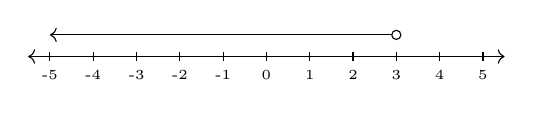
\begin{tikzpicture}[scale=0.55]
        \draw[<->] (-5.5,0) -- (5.5,0);
        \foreach \x in {-5,...,5} \draw (\x,0.1) -- (\x,-0.1) node[below] {\tiny \x};
        \draw (3,0.5) circle(3pt); \draw[->] (2.9,0.5)--(-5,0.5);
    \end{tikzpicture}
    \task\\
    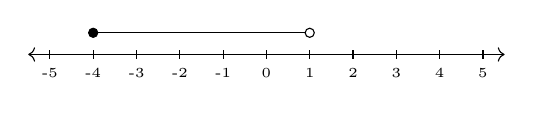
\begin{tikzpicture}[scale=0.55]
        \draw[<->] (-5.5,0) -- (5.5,0);
        \foreach \x in {-5,...,5} \draw (\x,0.1) -- (\x,-0.1) node[below] {\tiny \x};
        \filldraw (-4,0.5) circle(3pt); \draw (1,0.5) circle(3pt); \draw[] (-3.9,0.5)--(0.9,0.5);
    \end{tikzpicture}
\end{tasks}
\begin{solution}
    a) $(-\infty, 3)$ \\
    b) $[-4, 1)$
\end{solution}
\vspace{5mm} % Replaced \VSP[5]

\question Represent the following values on a number line.

\begin{tasks}(2)
    \task $x \in (-\infty, 2] \cup [4, \infty)$
    \\
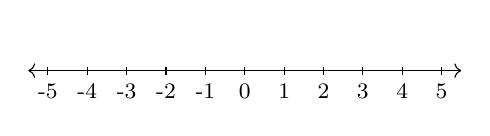
\begin{tikzpicture}[scale=0.5,baseline={([yshift=3ex]current bounding box.north)}]        
    \draw[<->] (-5.5,0) -- (5.5,0);
        \foreach \x in {-5,-4,-3,-2,-1,0,1,2,3,4,5} \draw (\x,0.1) -- (\x,-0.1) node[below] {\footnotesize \x};
    \end{tikzpicture}
    \task $\{x\in\mathbb{Z}\mid -4\leq x< 2\}$
    \\
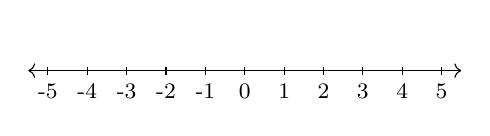
\begin{tikzpicture}[scale=0.5,baseline={([yshift=3ex]current bounding box.north)}]        
    \draw[<->] (-5.5,0) -- (5.5,0);
        \foreach \x in {-5,-4,-3,-2,-1,0,1,2,3,4,5} \draw (\x,0.1) -- (\x,-0.1) node[below] {\footnotesize \x};
    \end{tikzpicture}
\end{tasks}
\begin{solution}
\begin{tasks}(2)
    \task \\
    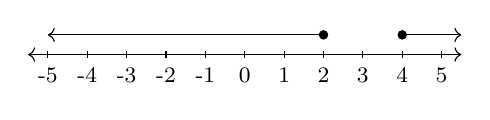
\begin{tikzpicture}[scale=0.5]
        \draw[<->] (-5.5,0) -- (5.5,0);
        \foreach \x in {-5,...,5} \draw (\x,0.1) -- (\x,-0.1) node[below] {\footnotesize \x};
        \filldraw (2,0.5) circle(3pt); \draw[->] (1.9,0.5)--(-5,0.5);
        \filldraw (4,0.5) circle(3pt); \draw[->] (4.1,0.5)--(5.5,0.5);
    \end{tikzpicture}
    \task \\
    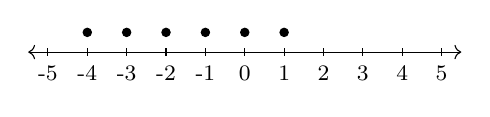
\begin{tikzpicture}[scale=0.5]
        \draw[<->] (-5.5,0) -- (5.5,0);
        \foreach \x in {-5,...,5} \draw (\x,0.1) -- (\x,-0.1) node[below] {\footnotesize \x};
        \foreach \p in {-4,-3,-2,-1,0,1} \filldraw (\p,0.5) circle (3pt);
    \end{tikzpicture}
\end{tasks}
\end{solution}

\question Solve the following. Express your final answer in \textbf{interval notation}.
\begin{tasks}(2)
    \task $5(x - 2) \geq 7x + 4$
    \task $x^2 + 5x + 6 > 0$
\end{tasks}
\begin{solution}
\begin{tasks}(2)
    \task $5x - 10 \geq 7x + 4 \implies -2x \geq 14 \implies x \leq -7$. Answer: $(-\infty, -7]$
    \task $(x+2)(x+3) > 0$. Roots at $-2, -3$. Check intervals. Answer: $(-\infty, -3) \cup (-2, \infty)$
\end{tasks}
\end{solution}
\vspace{\stretch{1}} % Replaced \svert

\question Sketch the solution region for the following inequalities.
\begin{tasks}(2)

    \task $y \geq \dfrac{2}{3}x - 2$ \\

     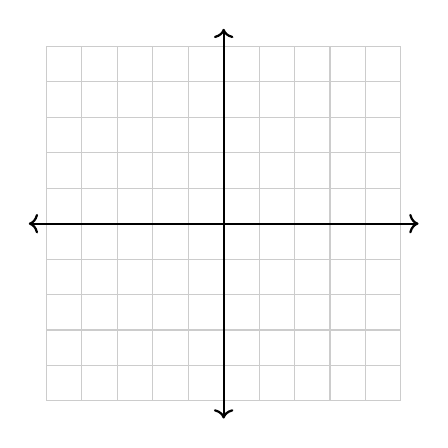
\begin{tikzpicture}[scale=0.45]

        \draw[opacity=0.2] (-5,-5) grid (5,5);

        \draw[<->,thick] (-5.5,0)--(5.5,0); \draw[<->,thick] (0,-5.5)--(0,5.5);

    \end{tikzpicture}

    \task $y < -(x + 3)^2 + 5$\\

    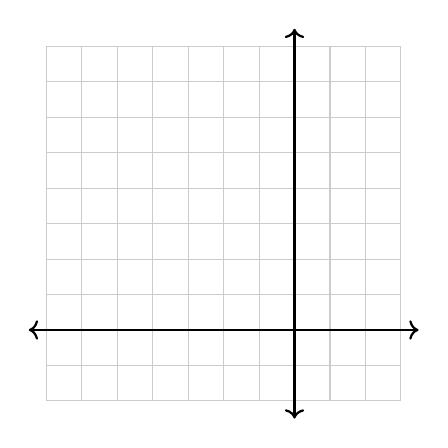
\begin{tikzpicture}[scale=0.45]

        \draw[opacity=0.2] (-7,-2) grid (3,8);

        \draw[<->,thick] (-7.5,0)--(3.5,0); \draw[<->,thick] (0,-2.5)--(0,8.5);

    \end{tikzpicture}

\end{tasks}
\begin{solution}
\begin{tasks}(2)
    \task Solid line, shade above. \\
    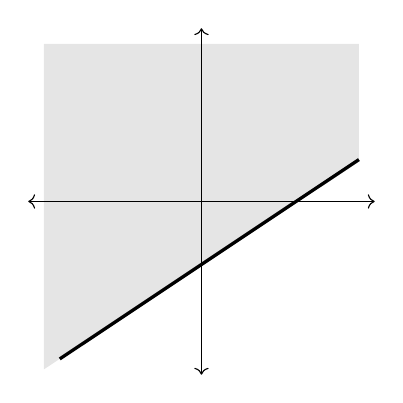
\begin{tikzpicture}[scale=0.4]
        \fill[gray!20] (-4.5,-5) -- (5,1.33) -- (5,5) -- (-5,5) -- (-5,-5.33) -- cycle;
        \draw[very thick] (-4.5,-5) -- (5,1.33);
        \draw[<->] (-5.5,0)--(5.5,0); \draw[<->] (0,-5.5)--(0,5.5);
    \end{tikzpicture}
    \task Dashed parabola, shade inside. \\
    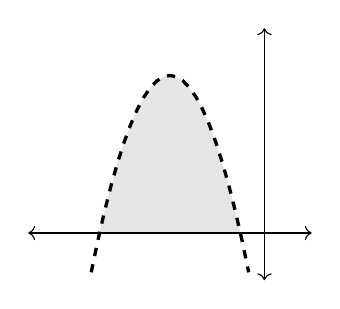
\begin{tikzpicture}[scale=0.4]
        \fill[gray!20, domain=-5.23:-0.76, variable=\x] 
            plot (\x, {-(\x+3)^2 + 5}) -- cycle;
        \draw[dashed, very thick, domain=-5.5:-0.5, variable=\x] plot (\x, {-(\x+3)^2 + 5});
        \draw[<->] (-7.5,0)--(1.5,0); \draw[<->] (0,-1.5)--(0,6.5);
    \end{tikzpicture}
\end{tasks}
\end{solution}

\pagebreak
\question Given $A=\{4,5,6,7,8\}$ and $B=\{3,6,7,9,10 \}$, find the following
\begin{tasks}(2)
    \task $A\cup B$ \task $A\cap B$
\end{tasks}
\begin{solution}
    a) $\{3, 4, 5, 6, 7, 8, 9, 10\}$ \\
    b) $\{6, 7\}$
\end{solution}
\vspace{0.5cm} % Replaced \svert[0.5]

\question Given $C=[-10,9)$ and $D=(-13,4]$, find the following
\begin{tasks}(2)
    \task $C\cup D$ \task $C\cap D$
\end{tasks}
\begin{solution}
    a) $(-13, 9)$ \\
    b) $[-10, 4]$
\end{solution}
\vspace{\stretch{1}} % Replaced \svert[1]

\subsection*{Level 3 to Level 4 Questions}

\question Solve the following one-variable inequalities algebraically. Express answers in \textbf{interval notation}.
    $$2x^2 - 7x - 4 \leq 0$$

\begin{solution}
    $(2x+1)(x-4) \leq 0$. Roots at $-0.5$ and $4$. Test $x=0$: $(1)(-4) = -4 \leq 0$ (True). Answer: $[-0.5, 4]$
\end{solution}
\vspace{\stretch{1.5}} % Replaced \svert[1.5]

\question Solve the following inequality for $x$:
\[ \dfrac{x^2 - x - 12}{x - 1} \leq 0 \]
\begin{solution}
    $\frac{(x-4)(x+3)}{x-1} \leq 0$. Critical values: $-3, 1$ (NPV), $4$. \\
    Sign Chart: $(-\infty, -3]: -$, $[-3, 1): +$, $(1, 4]: -$, $[4, \infty): +$. \\
    Final Answer: $(-\infty, -3] \cup (1, 4]$
\end{solution}
\vspace{\stretch{2}} % Replaced \svert[2]

\pagebreak

\question Graph the solution regions for the following quadratic inequalities in standard form.

\begin{tasks}(2)

    \task $y  <x^2 - 4x - 2$ \\[2ex]
    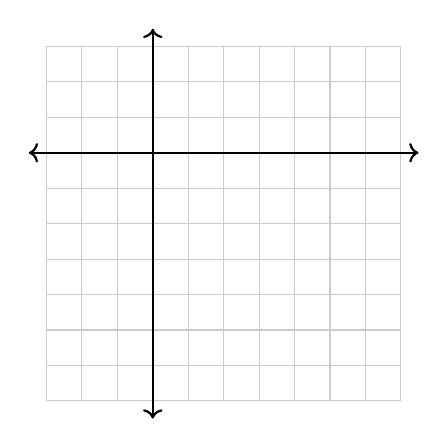
\begin{tikzpicture}[scale=0.45]
        \draw[opacity=0.2] (-3,-7) grid (7,3);
        \draw[<->,thick] (-3.5,0)--(7.5,0); \draw[<->,thick] (0,-7.5)--(0,3.5);
    \end{tikzpicture}
    \task \begin{cases}
        y \leq -x^2 + 6x - 4 \\
        y\geq \frac{1}{2}x-1
    \end{cases} \\
    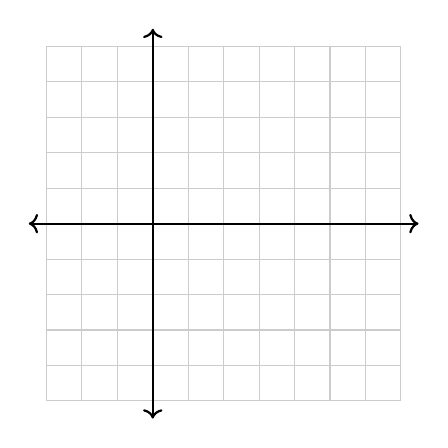
\begin{tikzpicture}[scale=0.45]
        \draw[opacity=0.2] (-3,-5) grid (7,5);
        \draw[<->,thick] (-3.5,0)--(7.5,0); \draw[<->,thick] (0,-5.5)--(0,5.5);
    \end{tikzpicture}
\end{tasks}

\vspace{\stretch{1}} % Replaced \svert

\question Write a two-variable inequality to represent the following shaded solution area.
   \begin{flushright}
        \begin{tikzpicture}[scale=0.5]
            \clip (-6.2,-6.2) rectangle (6.2,6.2);
            \fill[gray!30, domain=-3.16:3.16, variable=\x]
              (-2,4) -- plot ({\x}, {(\x-1)^2 - 5}) -- (2,-4) -- cycle;
            \draw[opacity=0.2] (-6,-6) grid (6,6);
            \draw[thick,<->] (-6.2,0)--(6.2,0); \draw[thick,<->] (0,-6.2)--(0,6.2);
            \draw[very thick, dashed, <->, domain=-2.3:4.3, variable=\x] plot ({\x}, {(\x-1)^2 - 5});
            \draw[very thick, <->] (-3,6)--(3,-6)
        \end{tikzpicture}
    \end{flushright}
\vspace{\stretch{1}} % Replaced \svert
\begin{solution}
    The dashed boundary is the parabola $y > (x-1)^2 - 5$. \\
    The solid boundary is the line $y \leq -2x$. \\
    System: $\{y > (x-1)^2 - 5, y \leq -2x\}$
\end{solution}
\vspace{\stretch{1}} % Replaced \svert
\pagebreak

% =========================================================
% LEVEL 5 TO LEVEL 6
% =========================================================
\subsection*{Level 5 to Level 6 Questions}
\question Solve the following inequalities.
\begin{tasks}(2)
    \task $4x^2-12x+9\leq0$ \task $x^2+1-(3x^2+4)<0$
\end{tasks}
\begin{solution}
\begin{tasks}(2)
    \task $(2x-3)^2 \leq 0$. $x = 1.5$.
    \task $-2x^2 - 3 < 0$. $(-\infty, \infty)$
\end{tasks}
\end{solution}
\vspace{\stretch{1}} % Replaced \svert

\question Solve for the value of $k$, if $4x^2-3kx+2=0$ were to have no real solutions.
\begin{solution}
    \[ (-3k)^2 - 4(4)(2) < 0 \implies 9k^2 - 32 < 0 \implies  k^2 < \frac{32}{9} \implies |k| < \sqrt{\frac{32}{9}}\implies |k| < \frac{4\sqrt{2}}{3} \]

    \textbf{Final Answer:} The equation has no real solutions when $\mathbf{-\dfrac{4\sqrt{2}}{3} < k < \dfrac{4\sqrt{2}}{3}}$ 
    (or approximately $-1.89 < k < 1.89$).
\end{solution}
\vspace{\stretch{1}} % Replaced \svert

\pagebreak
\question A rectangle has a length that is $3$ cm longer than its width. If the area of the rectangle must be \textbf{at most} $40$ cm$^2$, determine the possible range of values for the width. Use an inequality to solve.
\begin{solution}
    Let $w$ = width. $w(w+3) \leq 40 \implies w^2+3w-40 \leq 0 \implies (w+8)(w-5) \leq 0$.
    Algebraic solution: $[-8, 5]$. Physical solution: Width must be positive. Answer: $(0, 5]$
\end{solution}
\vspace{\stretch{2}} % Replaced \svert[2]

\question Solve the following inequality for $x$:
\[ \dfrac{x^2 + 7}{x^2 - 9} \geq 2 \]
\begin{solution}
    $\frac{x^2 + 7 - 2(x^2 - 9)}{x^2 - 9} \geq 0 \implies \frac{-x^2 + 25}{x^2 - 9} \geq 0 \implies \frac{-(x-5)(x+5)}{(x-3)(x+3)} \geq 0$. \\
    Critical points: $-5, -3, 3, 5$. \\
    Testing yields: $[-5, -3) \cup (3, 5]$
\end{solution}
\vspace{\stretch{2}} % Replaced \svert[2]

\pagebreak
% =========================================================
% LEVEL 7
% =========================================================
\subsection*{Level 7 Question}
\question Answer the following parts.
\begin{tasks}
    \task Given the area formula of a triangle is $A=\dfrac{1}{2}ab\sin C$, find the area where $x=5$ cm, $y= 4$ cm and $\theta=83^\circ$. Round final answers to two decimal spots. \\[2ex]
     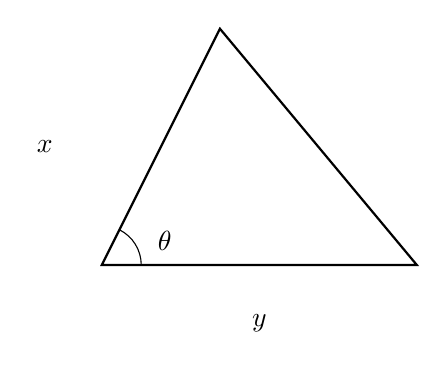
\begin{tikzpicture}[scale=1]
            % Replaced \drawanytriangle{4}{5}{6} with standard tikz triangle scaled to fit
            \coordinate (A) at (0,0);
            \coordinate (B) at (4,0);
            \coordinate (C) at (1.5, 3);
            \draw[thick] (A) -- (B) -- (C) -- cycle;
            % Replaced \labelside
            \node[left] at (-0.5, 1.5) {$x$};
            \node[below] at (2, -0.5) {$y$};
            % Replaced \tkzLabelAngle
            \tkzMarkAngle[size=0.5](B,A,C)
            \node at (0.8, 0.3) {$\theta$};
        \end{tikzpicture}
    \task Assume $x$ and $y$ are constant with the above values, for what values of $\theta$ would the area of the triangle be greater than $5$ cm$^2$?
\end{tasks}
\begin{solution}
\begin{tasks}
    \task $A = \dfrac{1}{2}(5)(4)\sin(83^\circ) = 10\sin(83^\circ) \approx \mathbf{9.93 \text{ cm}^2}$.
    \task We need to solve $10\sin\theta > 5$:
    \begin{flalign*}
        10\sin\theta &> 5 \\
        \sin\theta &> \frac{1}{2}
    \end{flalign*}
    The reference angle for $\sin\theta = \frac{1}{2}$ is $30^\circ$. In the context of a triangle, $\theta$ must be between $0^\circ$ and $180^\circ$. Sine is positive in both the first and second quadrants:
    \begin{itemize}
        \item Quadrant I: $\theta = 30^\circ$
        \item Quadrant II: $\theta = 180^\circ - 30^\circ = 150^\circ$
    \end{itemize}
    The area is greater than $5 \text{ cm}^2$ when $\mathbf{30^\circ < \theta < 150^\circ}$.
\end{tasks}
\end{solution}

\end{questions}
\end{document}